\documentclass{amsproc}
\usepackage{amssymb}
\usepackage{amsmath}
\usepackage{tikz}
\usepackage[siunitx, RPvoltages]{circuitikz}

\begin{document}

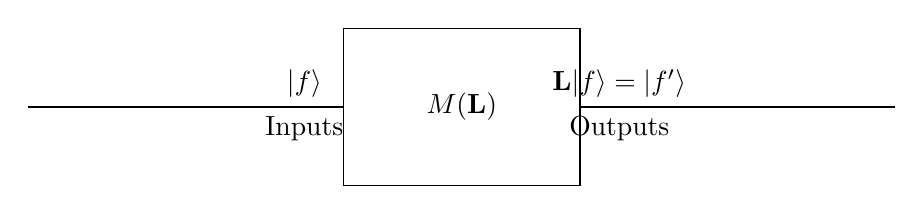
\begin{tikzpicture}
    % Create the main box for the computing machine
    \node[draw, rectangle, minimum width = 3 cm, minimum height = 2 cm] (fl) at (0,0) {$M(\mathbf{L})$};
    
    % Create the input line
    \draw[-] (fl.west) -- ++(-4,0);
    \node[above] at (-2,0) {$|f\rangle$};
    \node[below] at (-2,0) {Inputs};
    
    % Create the output line
    \draw[-] (fl.east) -- ++(4,0);
    \node[above] at (2,0) {$\mathbf{L}|f\rangle = |f'\rangle$};
    \node[below] at (2,0) {Outputs};
\end{tikzpicture}

\end{document}